% Neovim wall cheat sheet — A4 landscape, black & white.
% Build: /usr/local/texlive/2025/bin/x86_64-linux/lualatex nvim-cheatsheet.tex
\documentclass[10pt]{article}
\usepackage[a4paper,landscape,margin=7mm]{geometry}
\usepackage{fontspec}
\usepackage{xcolor}
\usepackage{tikz}
\usepackage{array}
\setlength{\parindent}{0pt}
\pagestyle{empty}

\setmainfont{Fira Sans}
\setmonofont{JetBrainsMono Nerd Font}[Scale=0.92]
\newfontfamily\headfont{Fira Sans}[UprightFont={* SemiBold}]

% ── building blocks ───────────────────────────────────────────────────────
% Section bar: solid black, white text. Prints crisply in B&W.
\newcommand{\sect}[1]{%
  \vspace{4.5pt}%
  \begin{tikzpicture}
    \node[fill=black, text=white, inner xsep=5pt, inner ysep=3.2pt,
          minimum width=\linewidth, anchor=west, align=left]
      {\headfont\fontsize{12.5}{12.5}\selectfont #1};
  \end{tikzpicture}\par
  \vspace{2.5pt}}

% One entry: bold mono key, sans description.
\newcommand{\kbd}[2]{%
  \begin{minipage}[t]{0.36\linewidth}\raggedright\ttfamily\bfseries\fontsize{11.5}{15}\selectfont #1\end{minipage}%
  \begin{minipage}[t]{0.64\linewidth}\raggedright\fontsize{10.5}{15}\selectfont #2\end{minipage}\par
  \vspace{2.4pt}}
% Wider key column for long combos.
\newcommand{\kbdw}[2]{%
  \begin{minipage}[t]{0.46\linewidth}\raggedright\ttfamily\bfseries\fontsize{11.5}{15}\selectfont #1\end{minipage}%
  \begin{minipage}[t]{0.54\linewidth}\raggedright\fontsize{10.5}{15}\selectfont #2\end{minipage}\par
  \vspace{2.4pt}}

\begin{document}

% ── title + the grammar ───────────────────────────────────────────────────
\begin{center}
  {\headfont\fontsize{22}{22}\selectfont NEOVIM}\hspace{14pt}%
  {\fontsize{13}{13}\selectfont move fast · edit precisely\hspace{10pt}·\hspace{10pt}{\ttfamily\bfseries C-}\,=\,Ctrl}\\[5pt]
  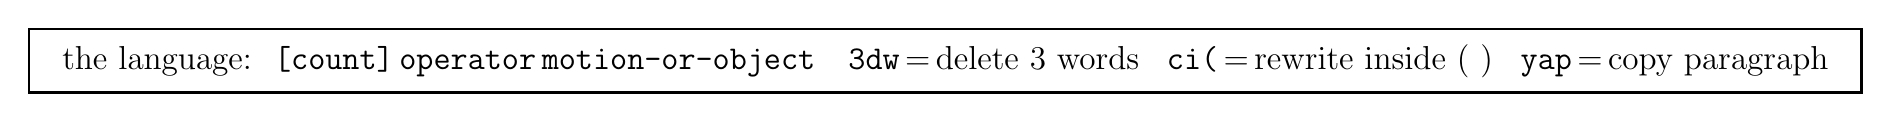
\begin{tikzpicture}
    \node[draw=black, line width=1pt, inner xsep=12pt, inner ysep=5.5pt] {%
      {\fontsize{12.5}{14}\selectfont
       the language:\hspace{8pt}{\ttfamily\bfseries [count]\,operator\,motion-or-object}%
       \hspace{12pt}{\ttfamily\bfseries 3dw}\,=\,delete 3 words%
       \hspace{10pt}{\ttfamily\bfseries ci(}\,=\,rewrite inside ( )%
       \hspace{10pt}{\ttfamily\bfseries yap}\,=\,copy paragraph}};
  \end{tikzpicture}
\end{center}
\vspace{1pt}

% ── four columns ──────────────────────────────────────────────────────────
\begin{minipage}[t]{0.24\textwidth}

\sect{WITHIN A LINE}
\kbd{f\,c\ \ t\,c}{jump onto / till before \texttt{c}}
\kbd{F\,c\ \ T\,c}{same, backwards}
\kbd{;\ \ ,}{repeat find / reverse it}
\kbd{0\ \ \^{}\ \ \$}{line start / first char / end}

\sect{BY WORD}
\kbd{w\ \ b}{next / previous word}
\kbd{e\ \ ge}{end of word, fwd / back}
\kbd{W\ B\ E}{same, space-separated}

\sect{BY BLOCK}
\kbd{\{\ \ \}}{paragraph up / down}
\kbd{\%}{matching \texttt{( ) [ ] \{ \}}}

\sect{INSERT — WHERE IT COUNTS}
\kbd{i\ \ a}{insert before / after}
\kbd{I\ \ A}{insert at line start / end}
\kbd{o\ \ O}{open line below / above}
\kbd{gi}{insert at last edit spot}

\end{minipage}\hfill
\begin{minipage}[t]{0.24\textwidth}

\sect{SCREEN \& FILE}
\kbd{gg\ \ G}{top / bottom of file}
\kbd{42G}{go to line 42}
\kbd{H\ M\ L}{screen top / mid / bottom}
\kbd{C-d\ \ C-u}{half page down / up}
\kbd{zz}{center the cursor line}

\sect{SEARCH}
\kbd{/text}{search forward (\texttt{?} = back)}
\kbd{n\ \ N}{next / previous match}
\kbd{*\ \ \#}{search word under cursor}

\sect{JUMPS \& MARKS}
\kbd{C-o\ \ C-i}{back / fwd in jump list}
\kbd{ma\ \ `a}{set mark a / jump to it}
\kbd{``}{back to pre-jump spot}
\kbd{gd}{go to definition}

\sect{COUNTS WORK EVERYWHERE}
\kbd{5j\ \ 3w\ \ 2\}}{multiply any motion}

\end{minipage}\hfill
\begin{minipage}[t]{0.24\textwidth}

\sect{OPERATORS\ \ (verb + motion)}
\kbd{d\ \ c\ \ y}{delete / change / yank}
\kbd{>\ \ <\ \ =}{indent right / left / auto}
\kbd{gu\ \ gU}{lowercase / UPPERCASE}

\sect{TEXT OBJECTS\ \ (after d c y v)}
\kbd{iw\ \ aw}{word / word + space}
\kbd{i"\ \ i'}{inside quotes}
\kbd{i(\ \ i\{\ \ i[}{inside brackets}
\kbd{a(\ \ a"}{…including the pair}
\kbd{ip\ \ ap}{paragraph}
\kbd{it\ \ at}{inside / around HTML tag}

\sect{THE MONEY COMBOS}
\kbdw{ciw}{rewrite word at cursor}
\kbdw{ci"\ \ ci(}{rewrite string / args}
\kbdw{dap}{delete paragraph}
\kbdw{yiw\ then\ viwp}{copy word, paste over}
\kbdw{.}{repeat last change}

\sect{POWER}
\kbd{qa\,…\,q\ \ @a}{record / play macro}
\kbd{"+y\ \ "+p}{system clipboard y / p}
\kbdw{:\%s/old/new/g}{replace in whole file}

\end{minipage}\hfill
\begin{minipage}[t]{0.24\textwidth}

\sect{LINE \& CHAR EDITS}
\kbd{dd\ \ yy\ \ cc}{del / copy / change line}
\kbd{D\ \ C\ \ Y}{same, cursor to line end}
\kbd{x\ \ r\,c\ \ s}{del char / replace / subst}
\kbd{J}{join with line below}
\kbd{p\ \ P}{paste after / before}
\kbd{u\ \ C-r}{undo / redo}
\kbd{C-a\ \ C-x}{number +1 / −1}

\sect{VISUAL MODE}
\kbd{v\ \ V\ \ C-v}{char / line / block}
\kbd{o}{to other end of selection}
\kbd{gv}{reselect last selection}
\kbd{C-v\,→\,I}{multi-line insert}

\sect{THIS CONFIG}
\kbd{C-scroll}{font size (\texttt{C-0} reset)}
\kbd{C-1\,…\,5}{pick one of five fonts}
\kbd{C-8\ \ C-9}{cycle nacre themes}
\kbd{C-q}{save everything \& quit}
\kbd{nvim}{bare start = last session}
\kbd{Space}{leader: LazyVim actions}

\end{minipage}

\end{document}
